\section{Formación de imágenes satelitales}
\subsection{Partes de una imagen}

\begin{frame}{\secname : \subsecname}
  \begin{figure}
    \centering
    %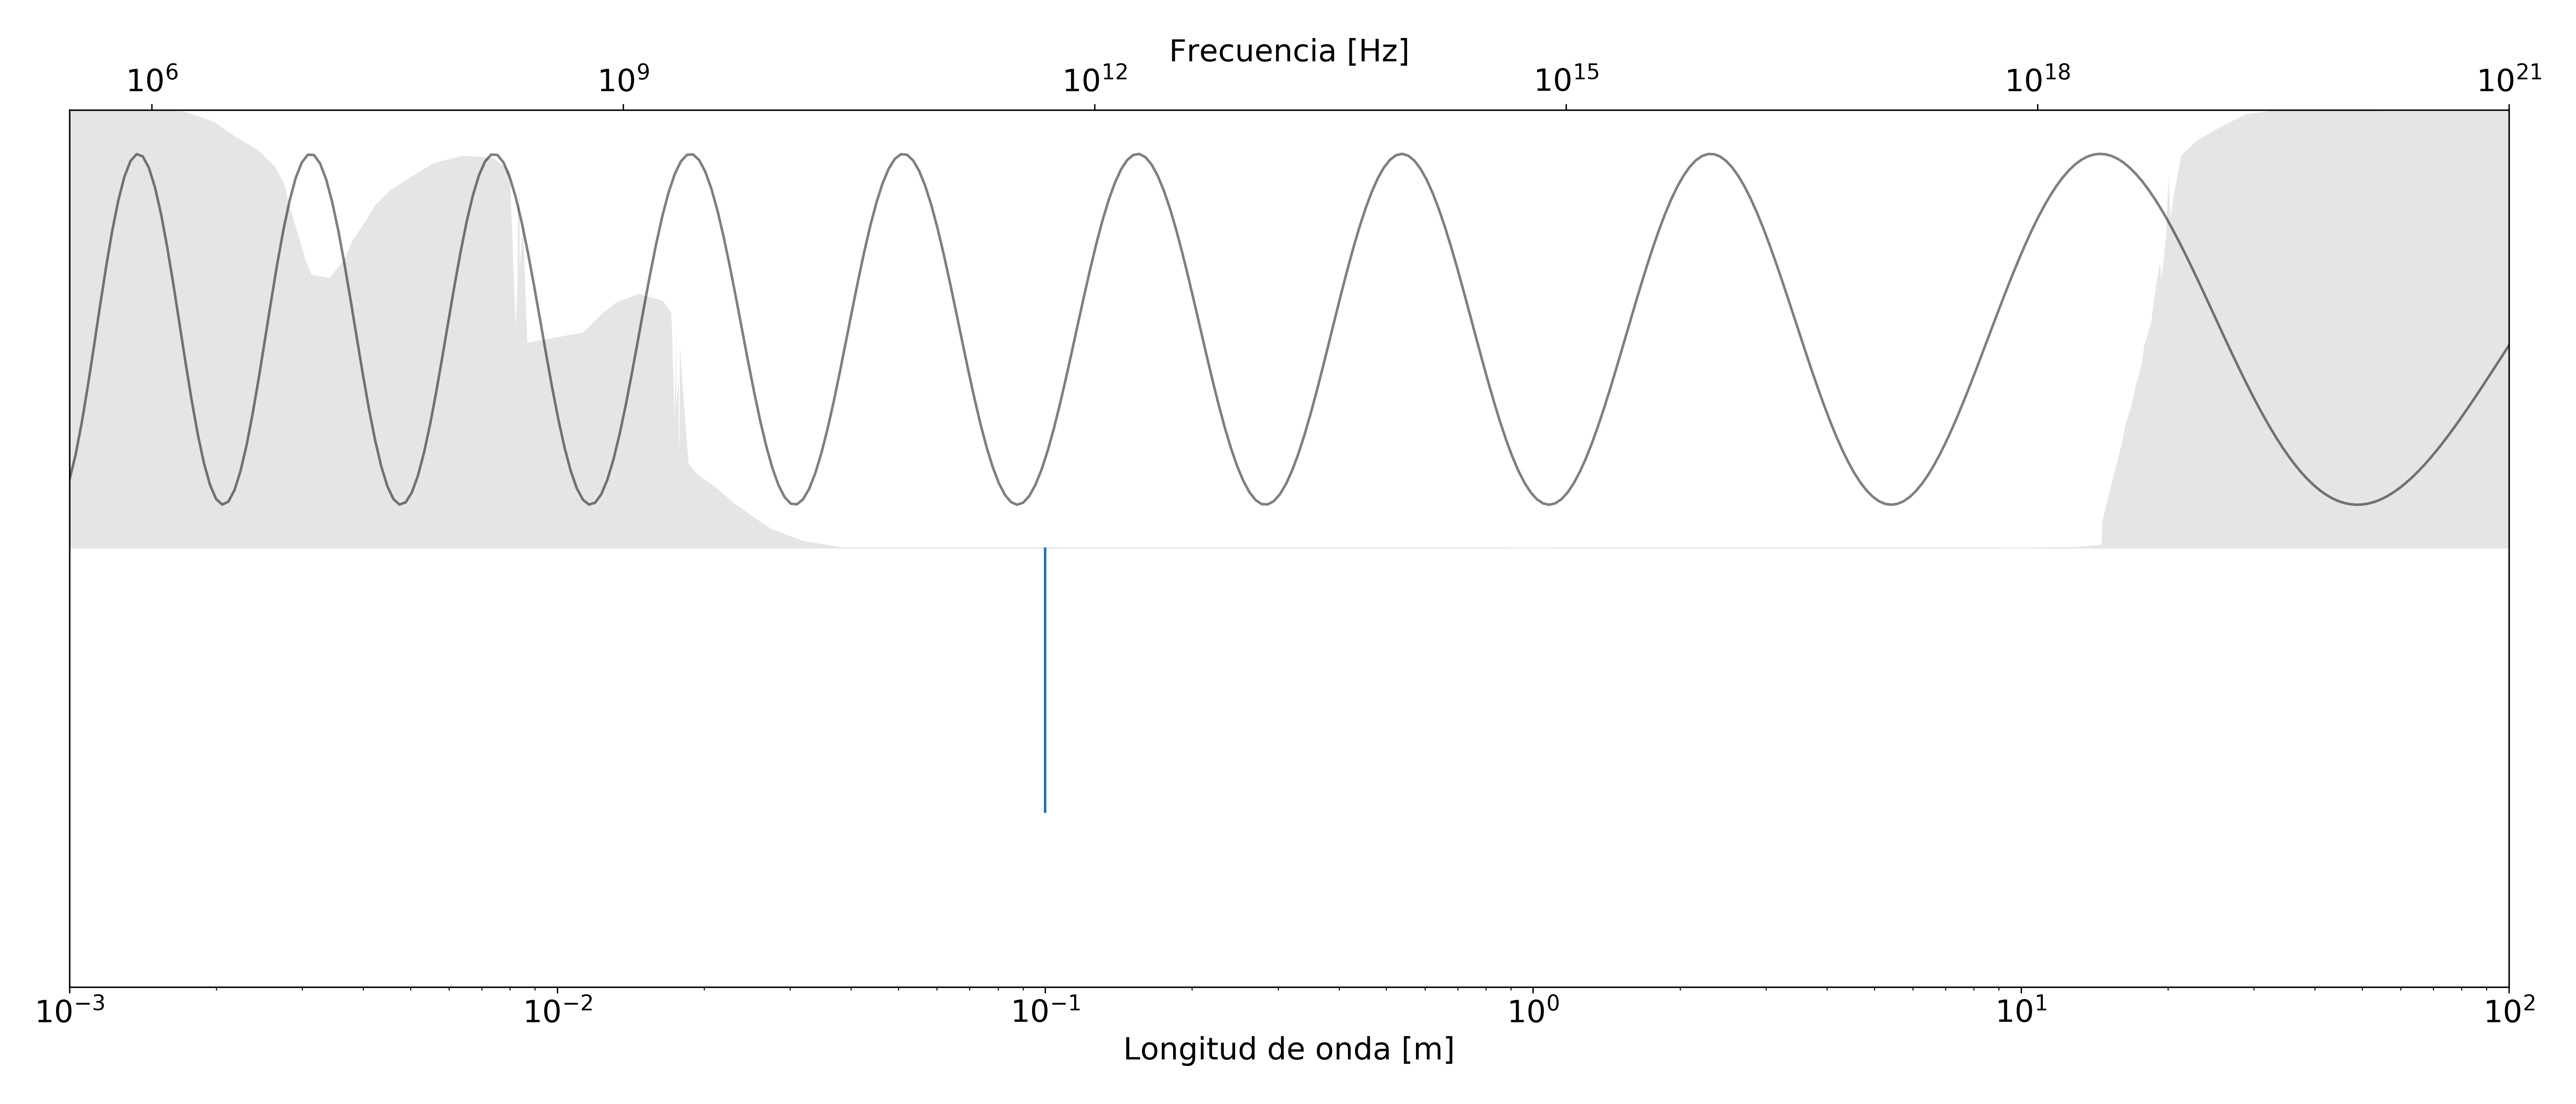
\includegraphics[width=\textwidth]{fig:espectro.png}
    \caption{Formación de un píxel.}
    \label{}
  \end{figure}
\end{frame}
%--- Next Frame ---%

\begin{frame}{\secname : \subsecname}
  \begin{figure}
    \centering
    %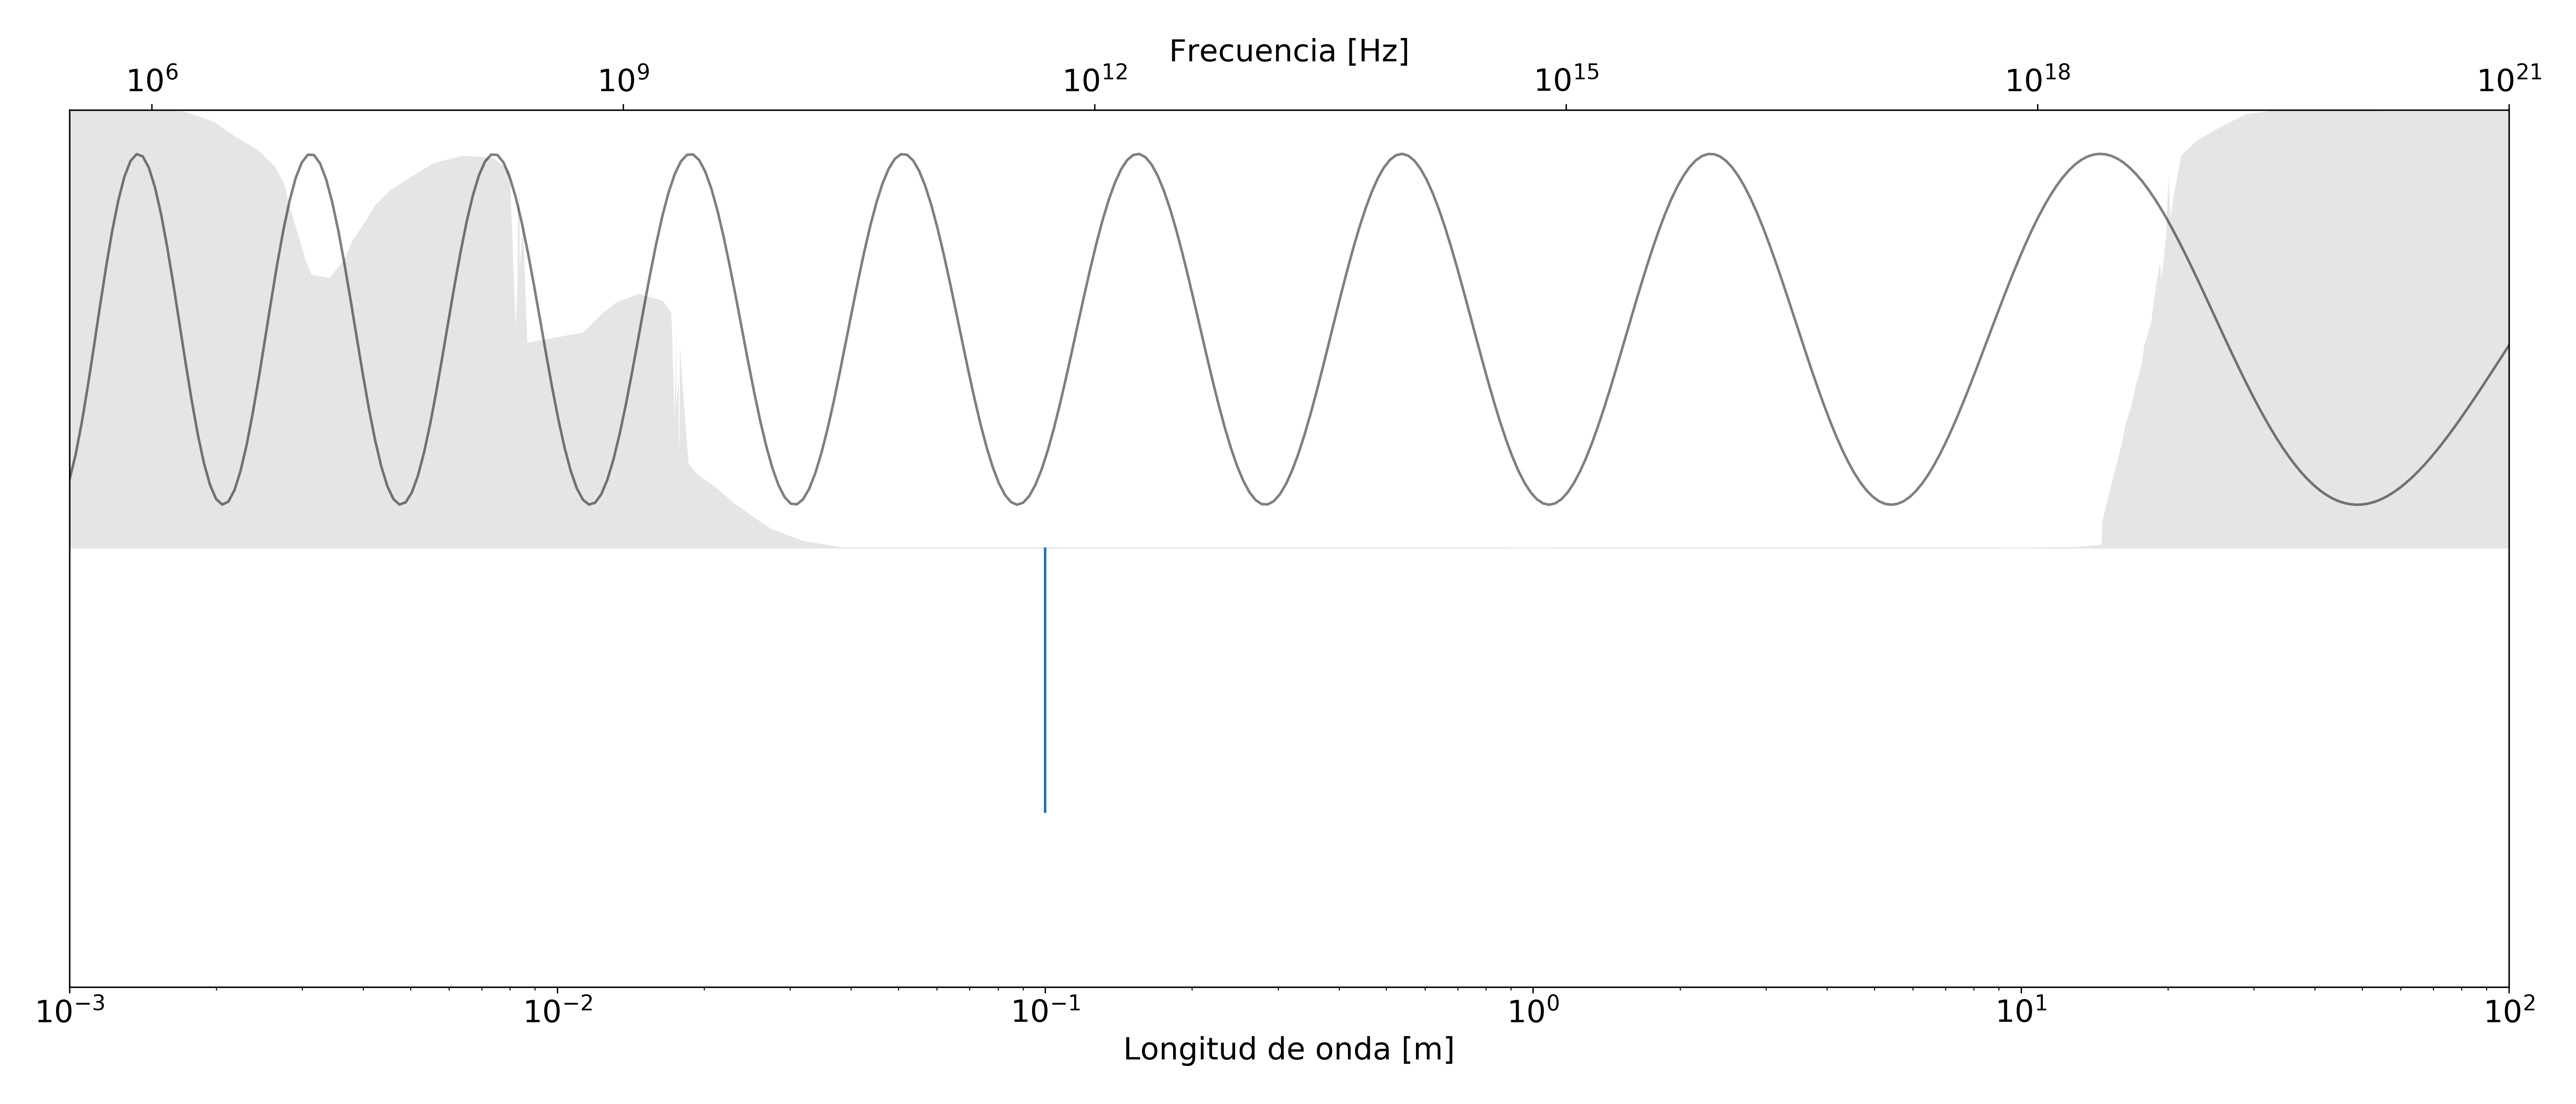
\includegraphics[width=\textwidth]{fig:espectro.png}
    \caption{Concepto de píxel.}
    \label{}
  \end{figure}
\end{frame}
%--- Next Frame ---%

\begin{frame}{\secname : \subsecname}
  \begin{figure}
    \centering
    %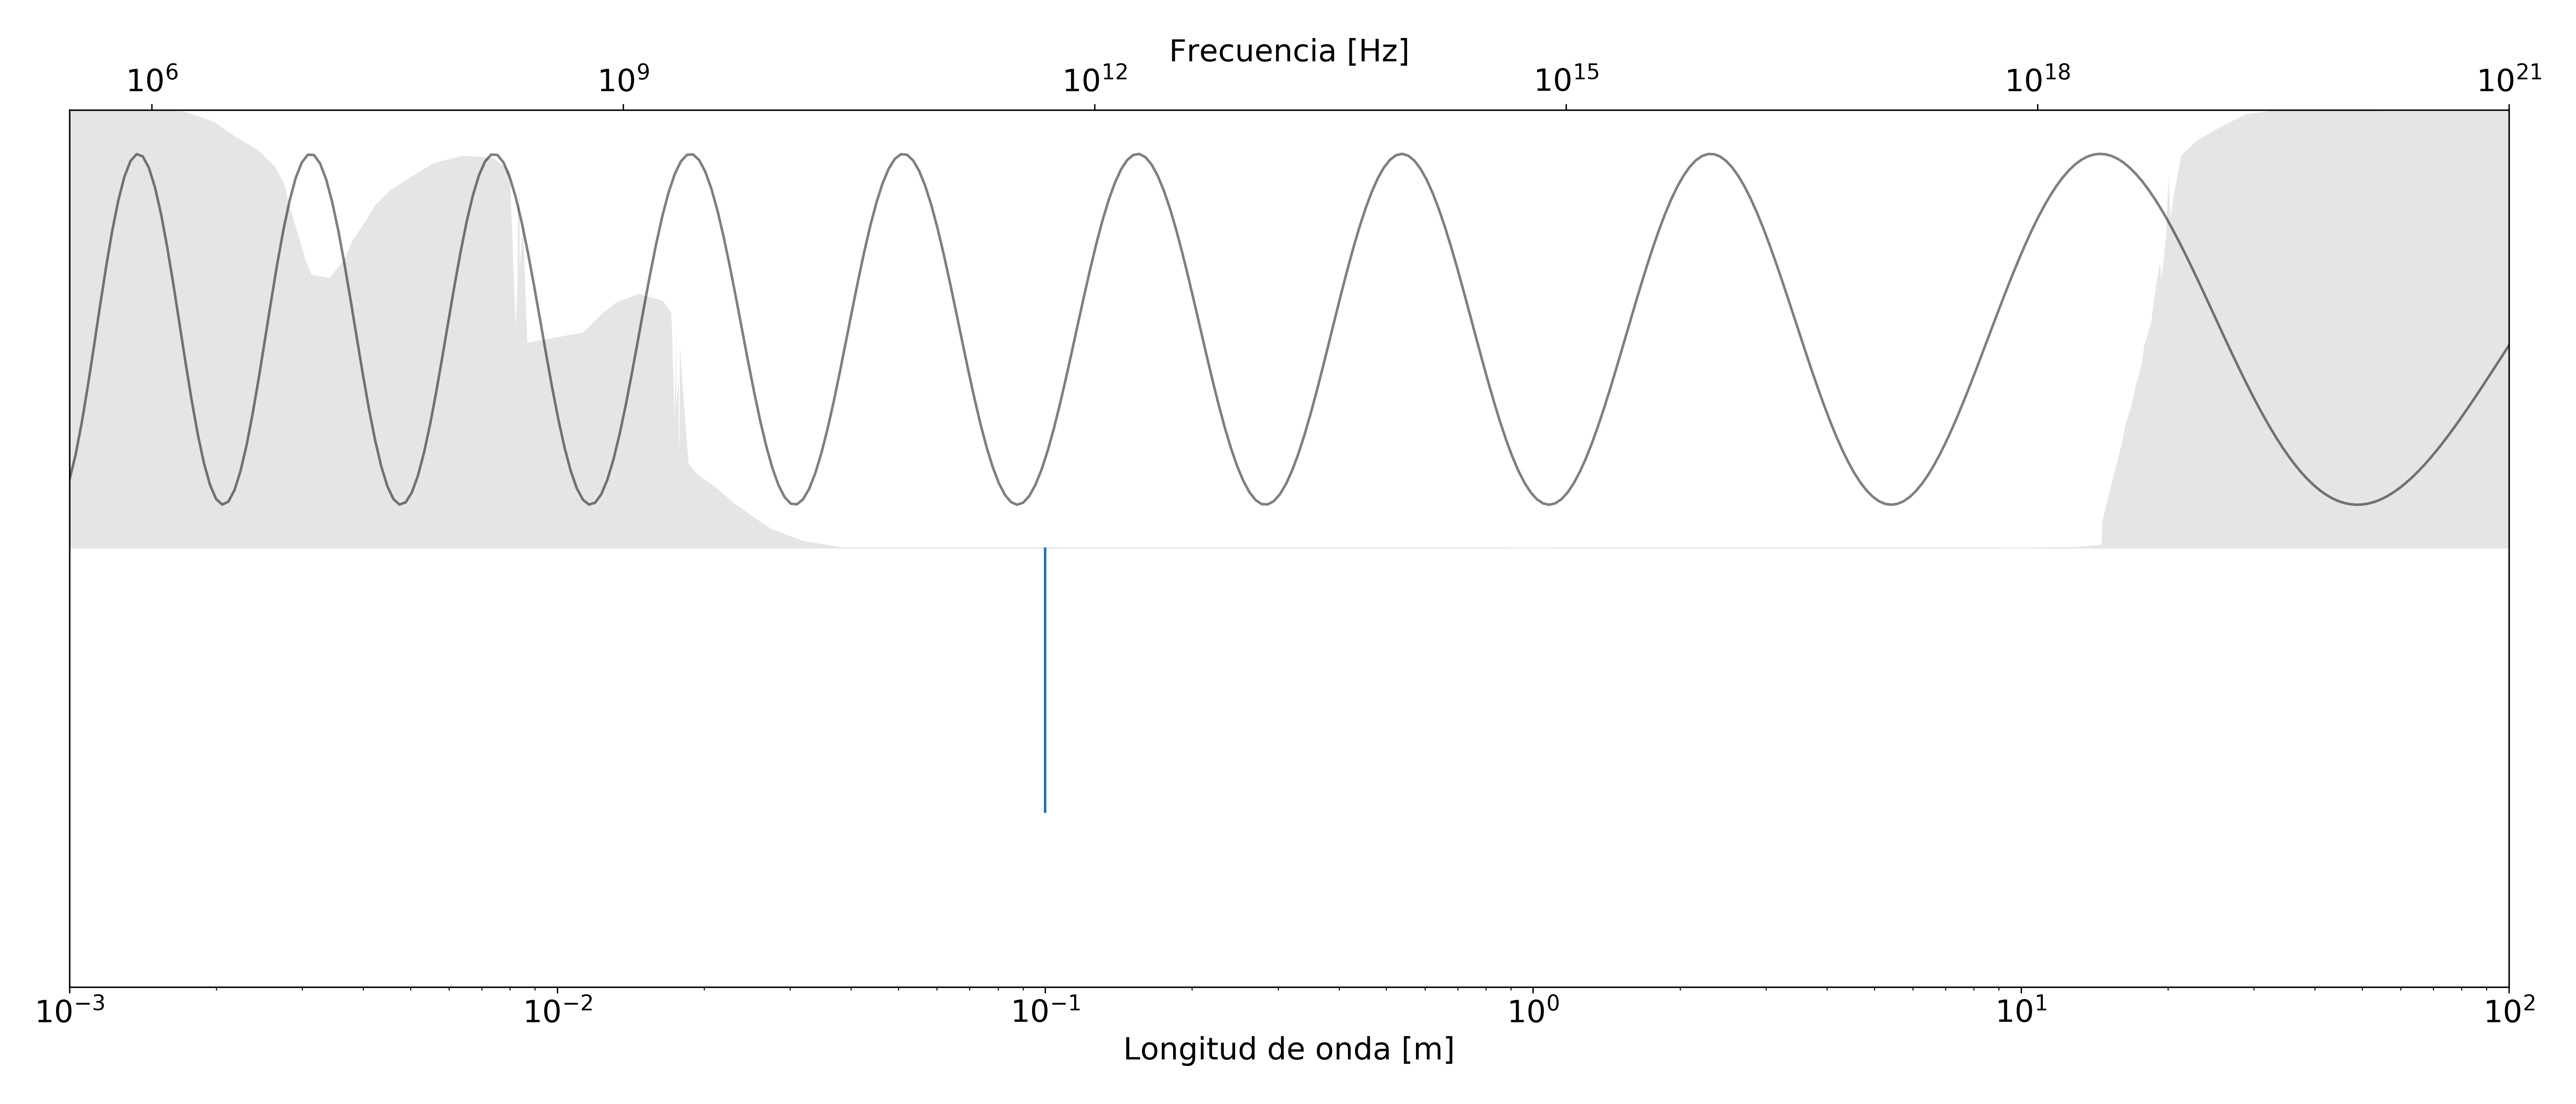
\includegraphics[width=\textwidth]{fig:espectro.png}
    \caption{Formación de una banda.}
    \label{}
  \end{figure}
\end{frame}
%--- Next Frame ---%

\begin{frame}{\secname : \subsecname}
  \begin{figure}
    \centering
    %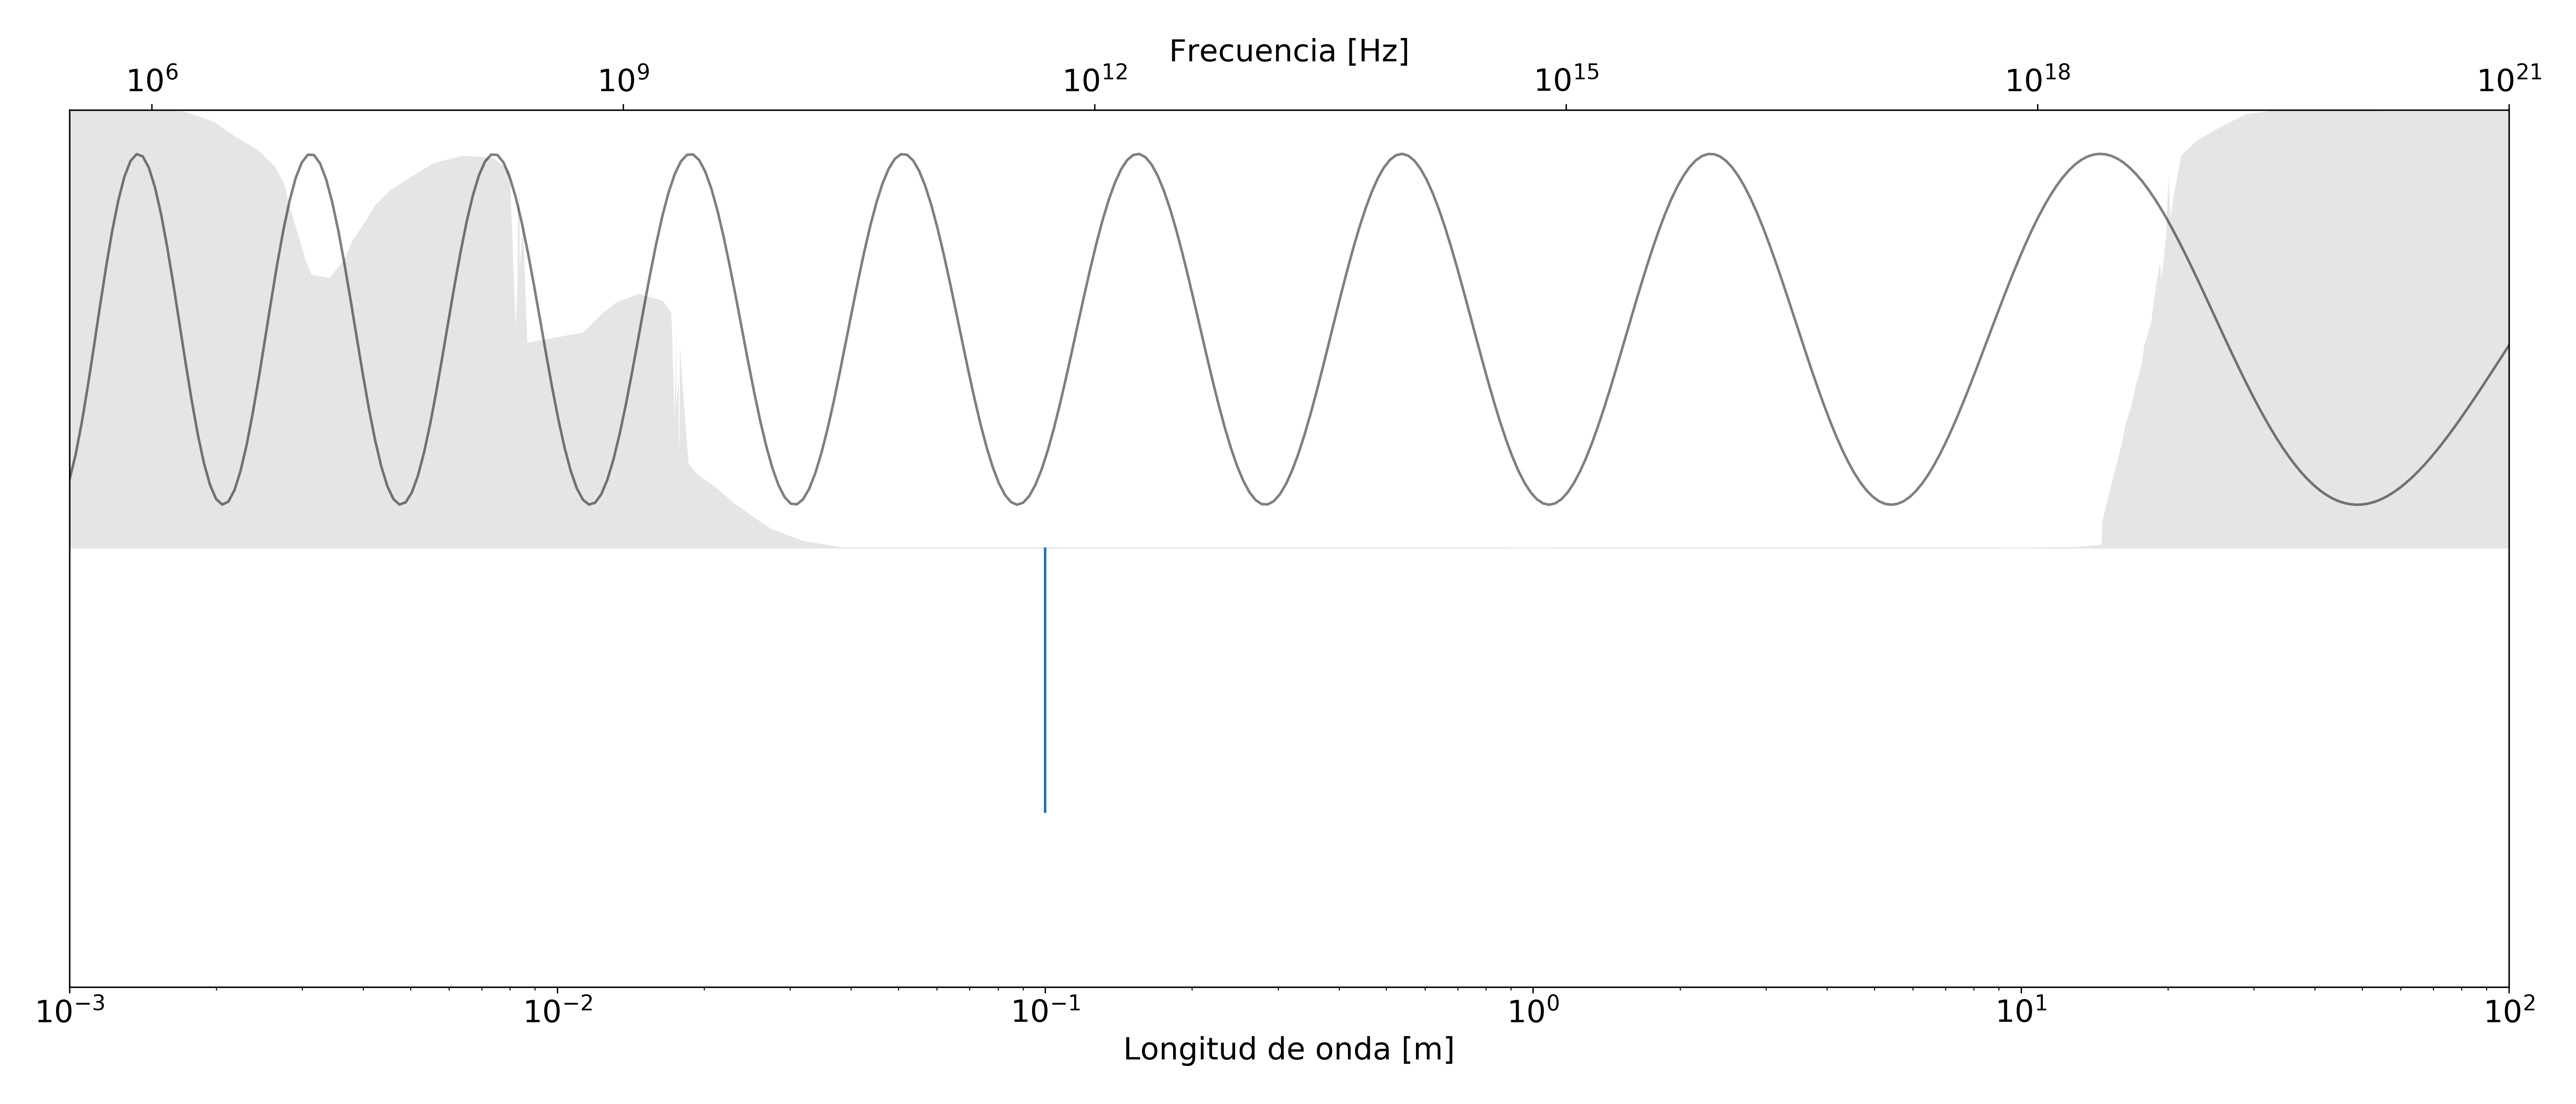
\includegraphics[width=\textwidth]{fig:espectro.png}
    \caption{Concepto de banda.}
    \label{}
  \end{figure}
\end{frame}
%--- Next Frame ---%

\begin{frame}{\secname : \subsecname}
  \begin{figure}
    \centering
    %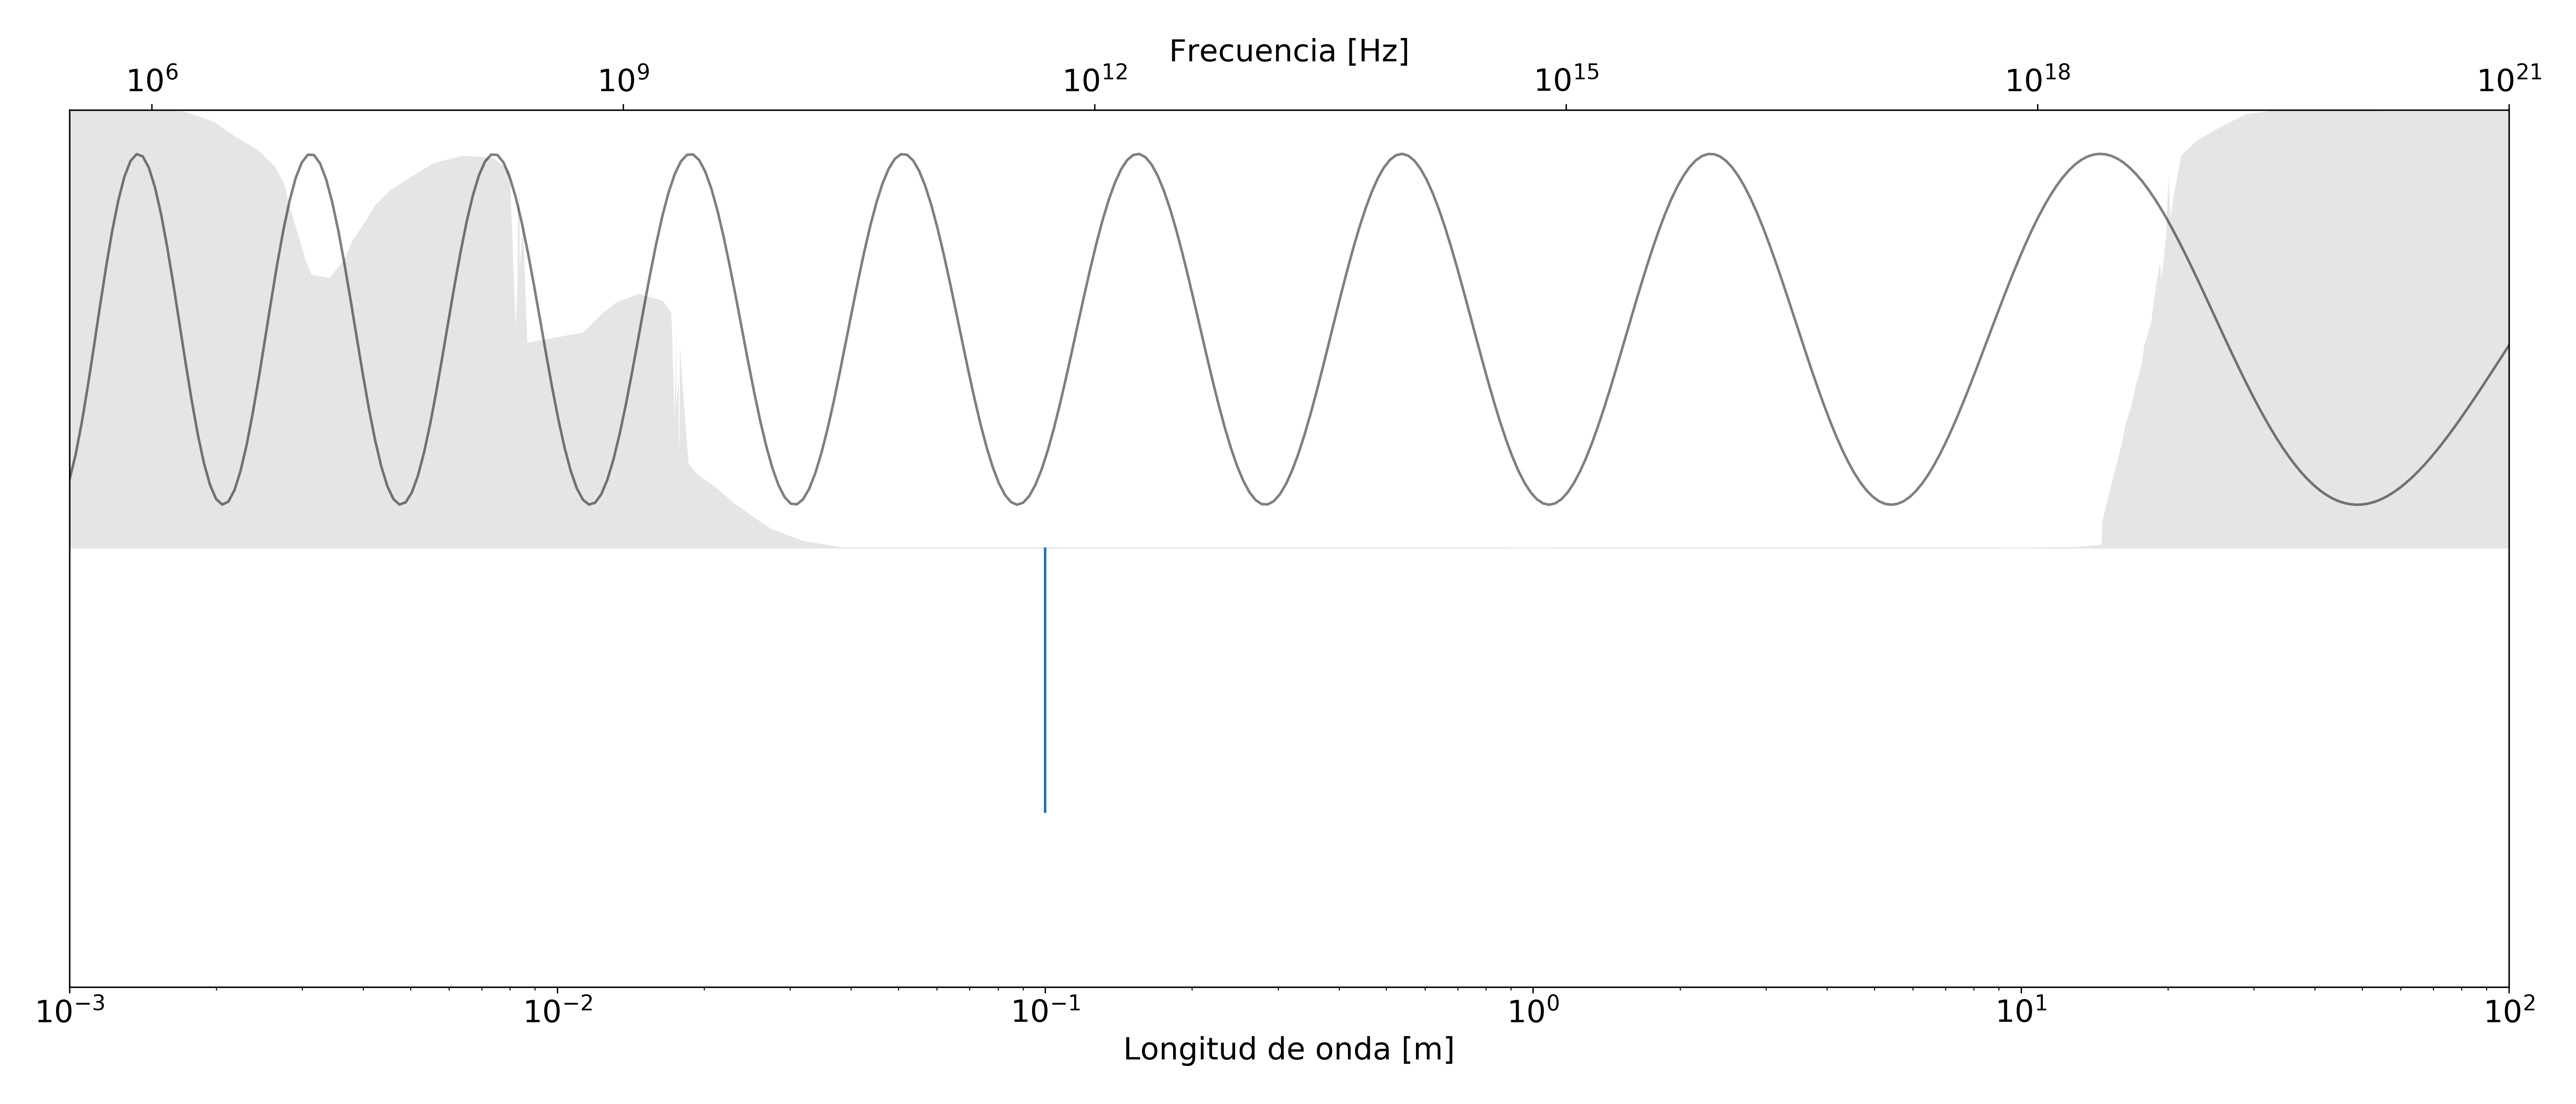
\includegraphics[width=\textwidth]{fig:espectro.png}
    \caption{Imagen raster como arreglo de píxeles y bandas.}
    \label{}
  \end{figure}
\end{frame}
%--- Next Frame ---%

\subsection{Resolución espectral y radiométrica}

\begin{frame}{\secname : \subsecname}
  \begin{figure}
    \centering
    %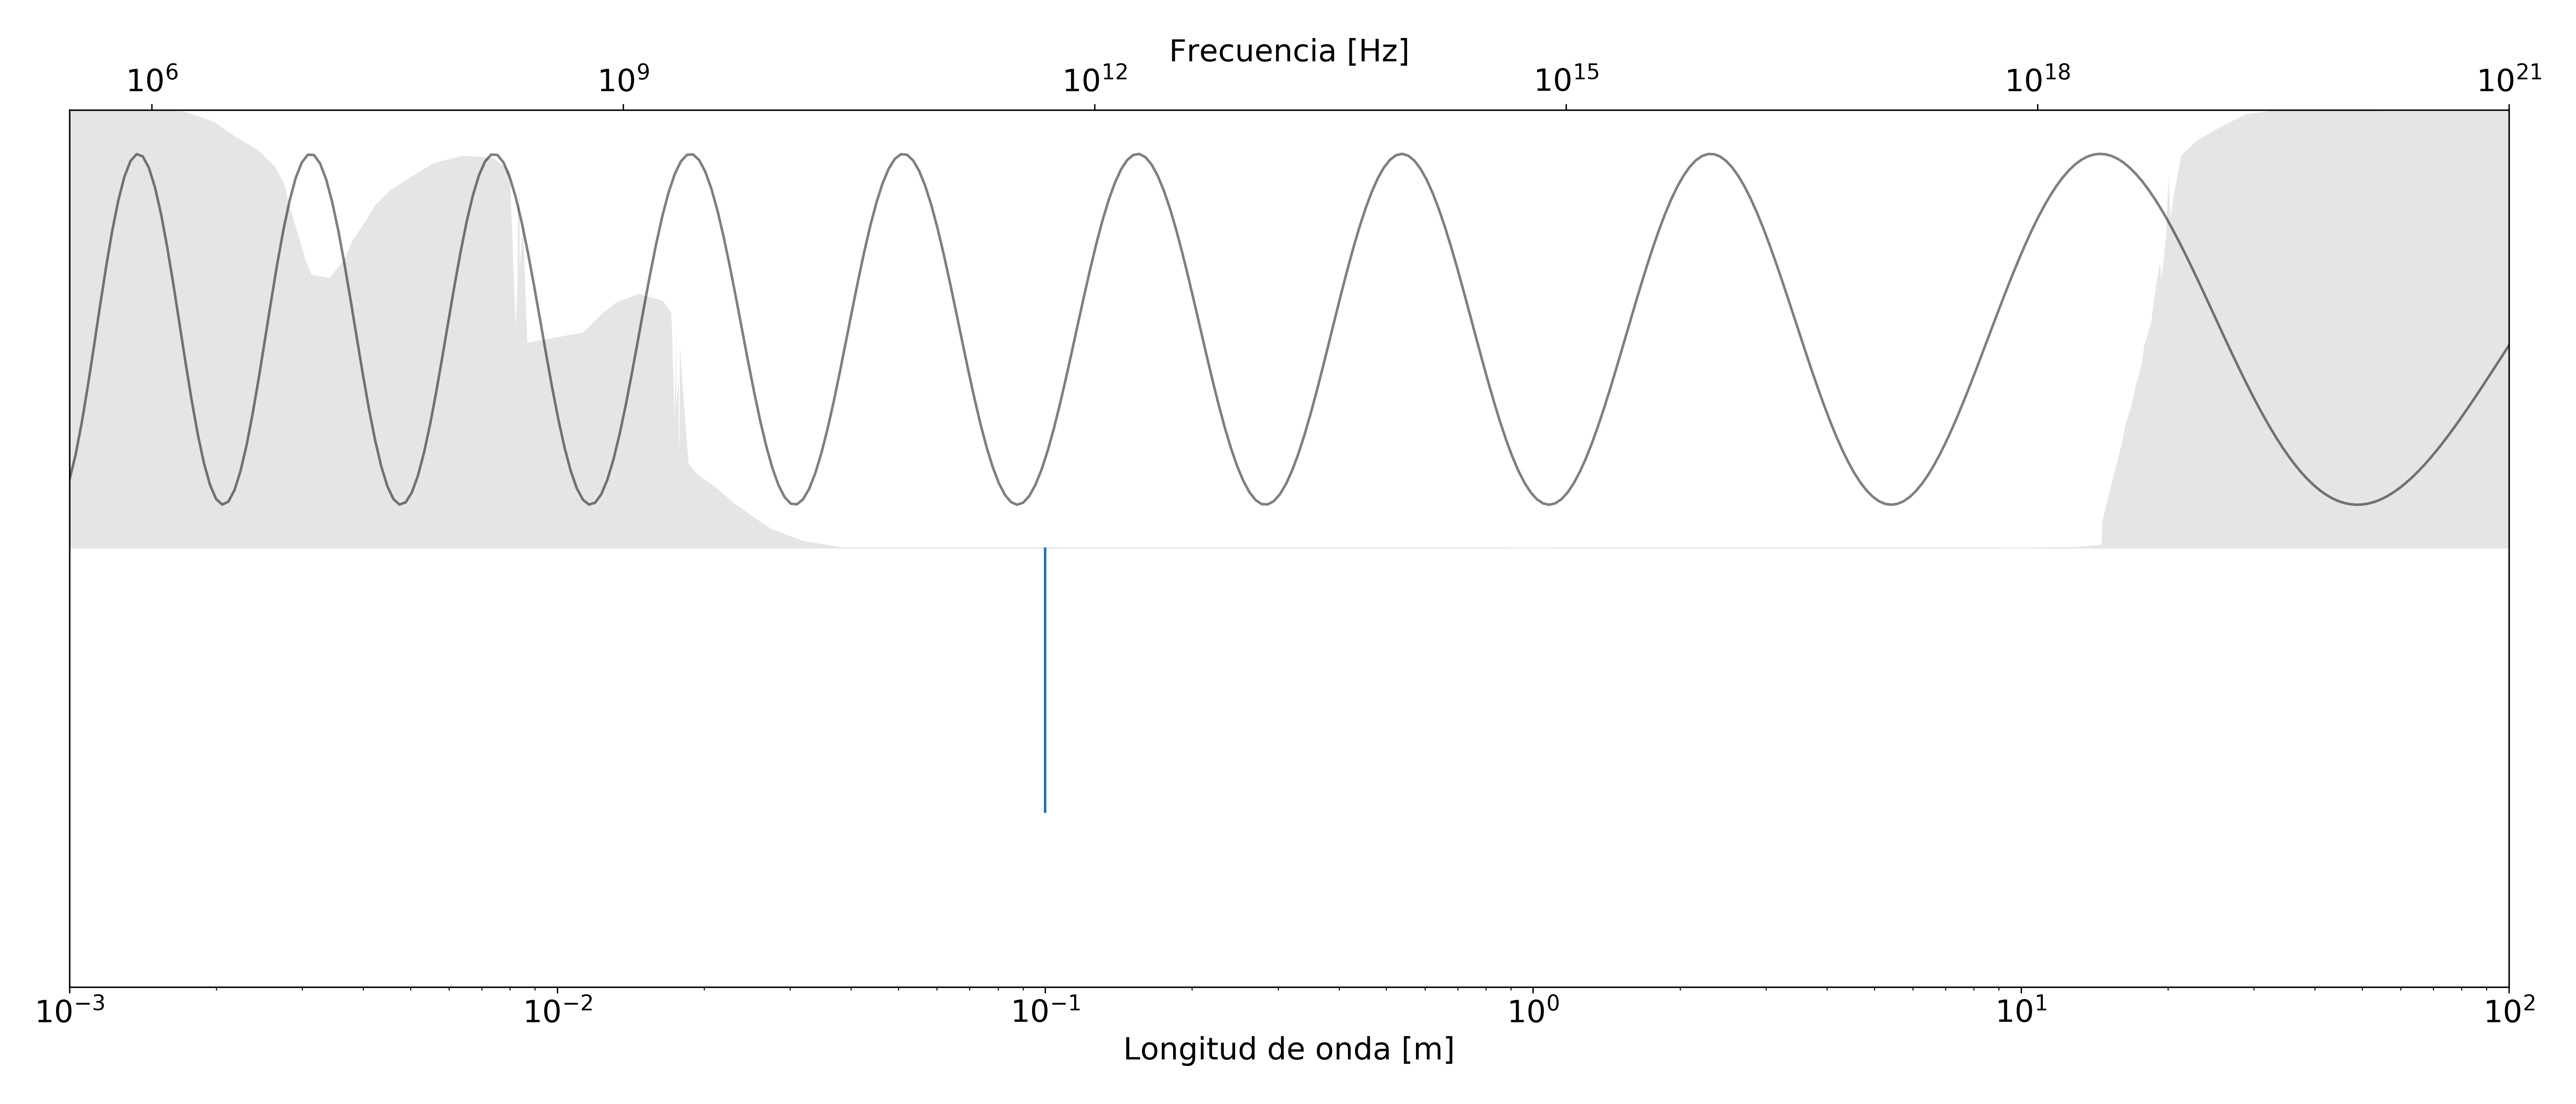
\includegraphics[width=\textwidth]{fig:espectro.png}
    \caption{Resolución radiométrica sobre la firma espectral.}
    \label{}
  \end{figure}
\end{frame}
%--- Next Frame ---%

\begin{frame}{\secname : \subsecname}
  \begin{figure}
    \centering
    %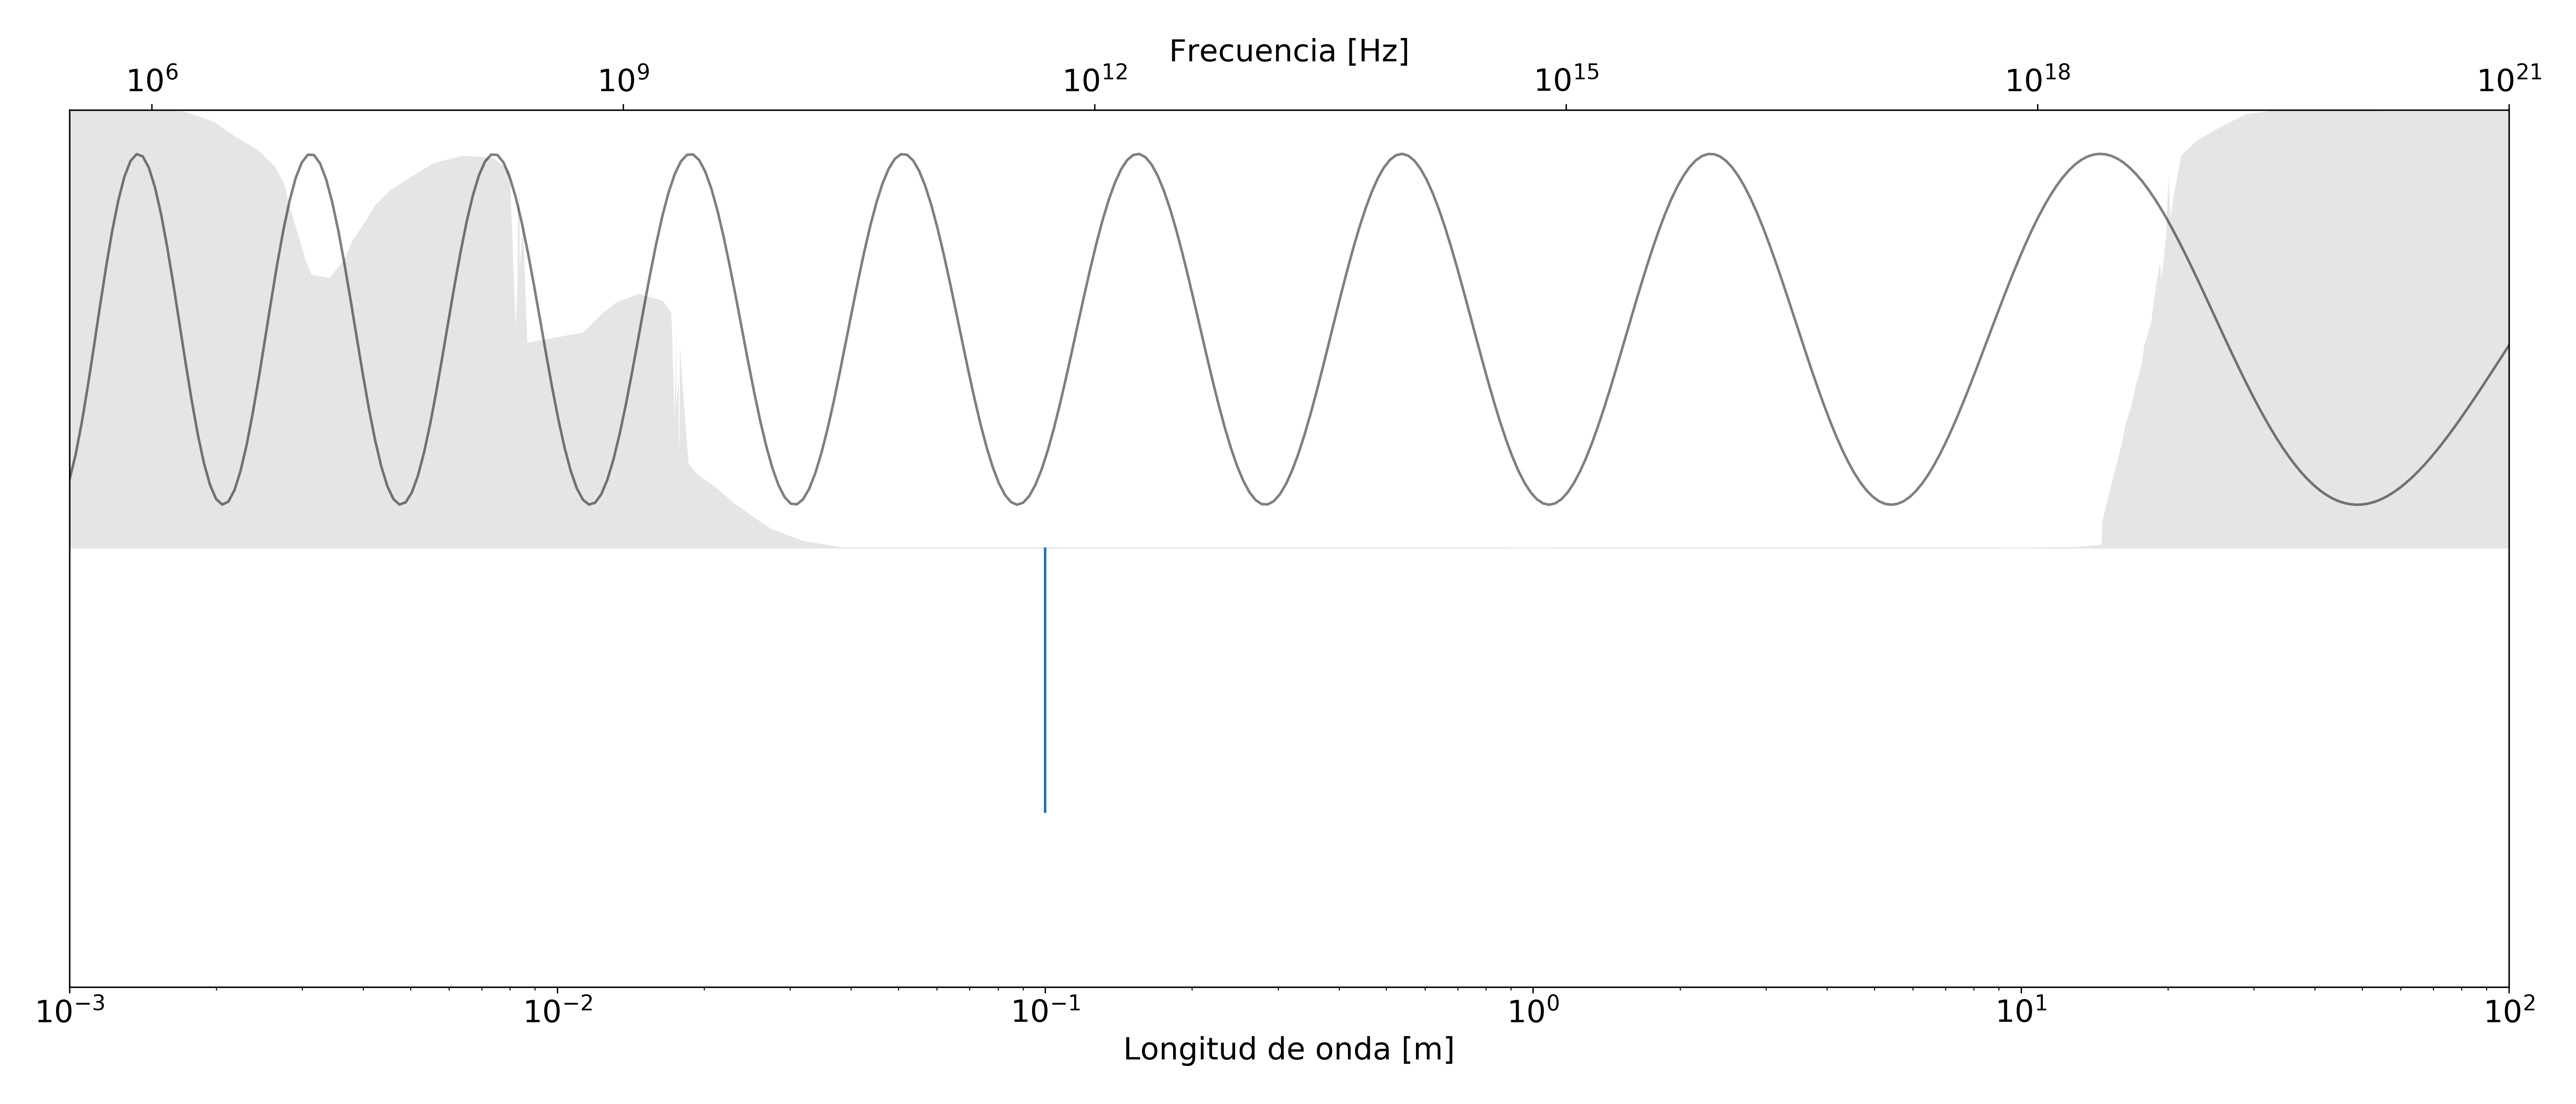
\includegraphics[width=\textwidth]{fig:espectro.png}
    \caption{Comparación de imágnes con distintas resoluciones radiométricas.}
    \label{}
  \end{figure}
\end{frame}
%--- Next Frame ---%

\begin{frame}{\secname : \subsecname}
  \begin{figure}
    \centering
    %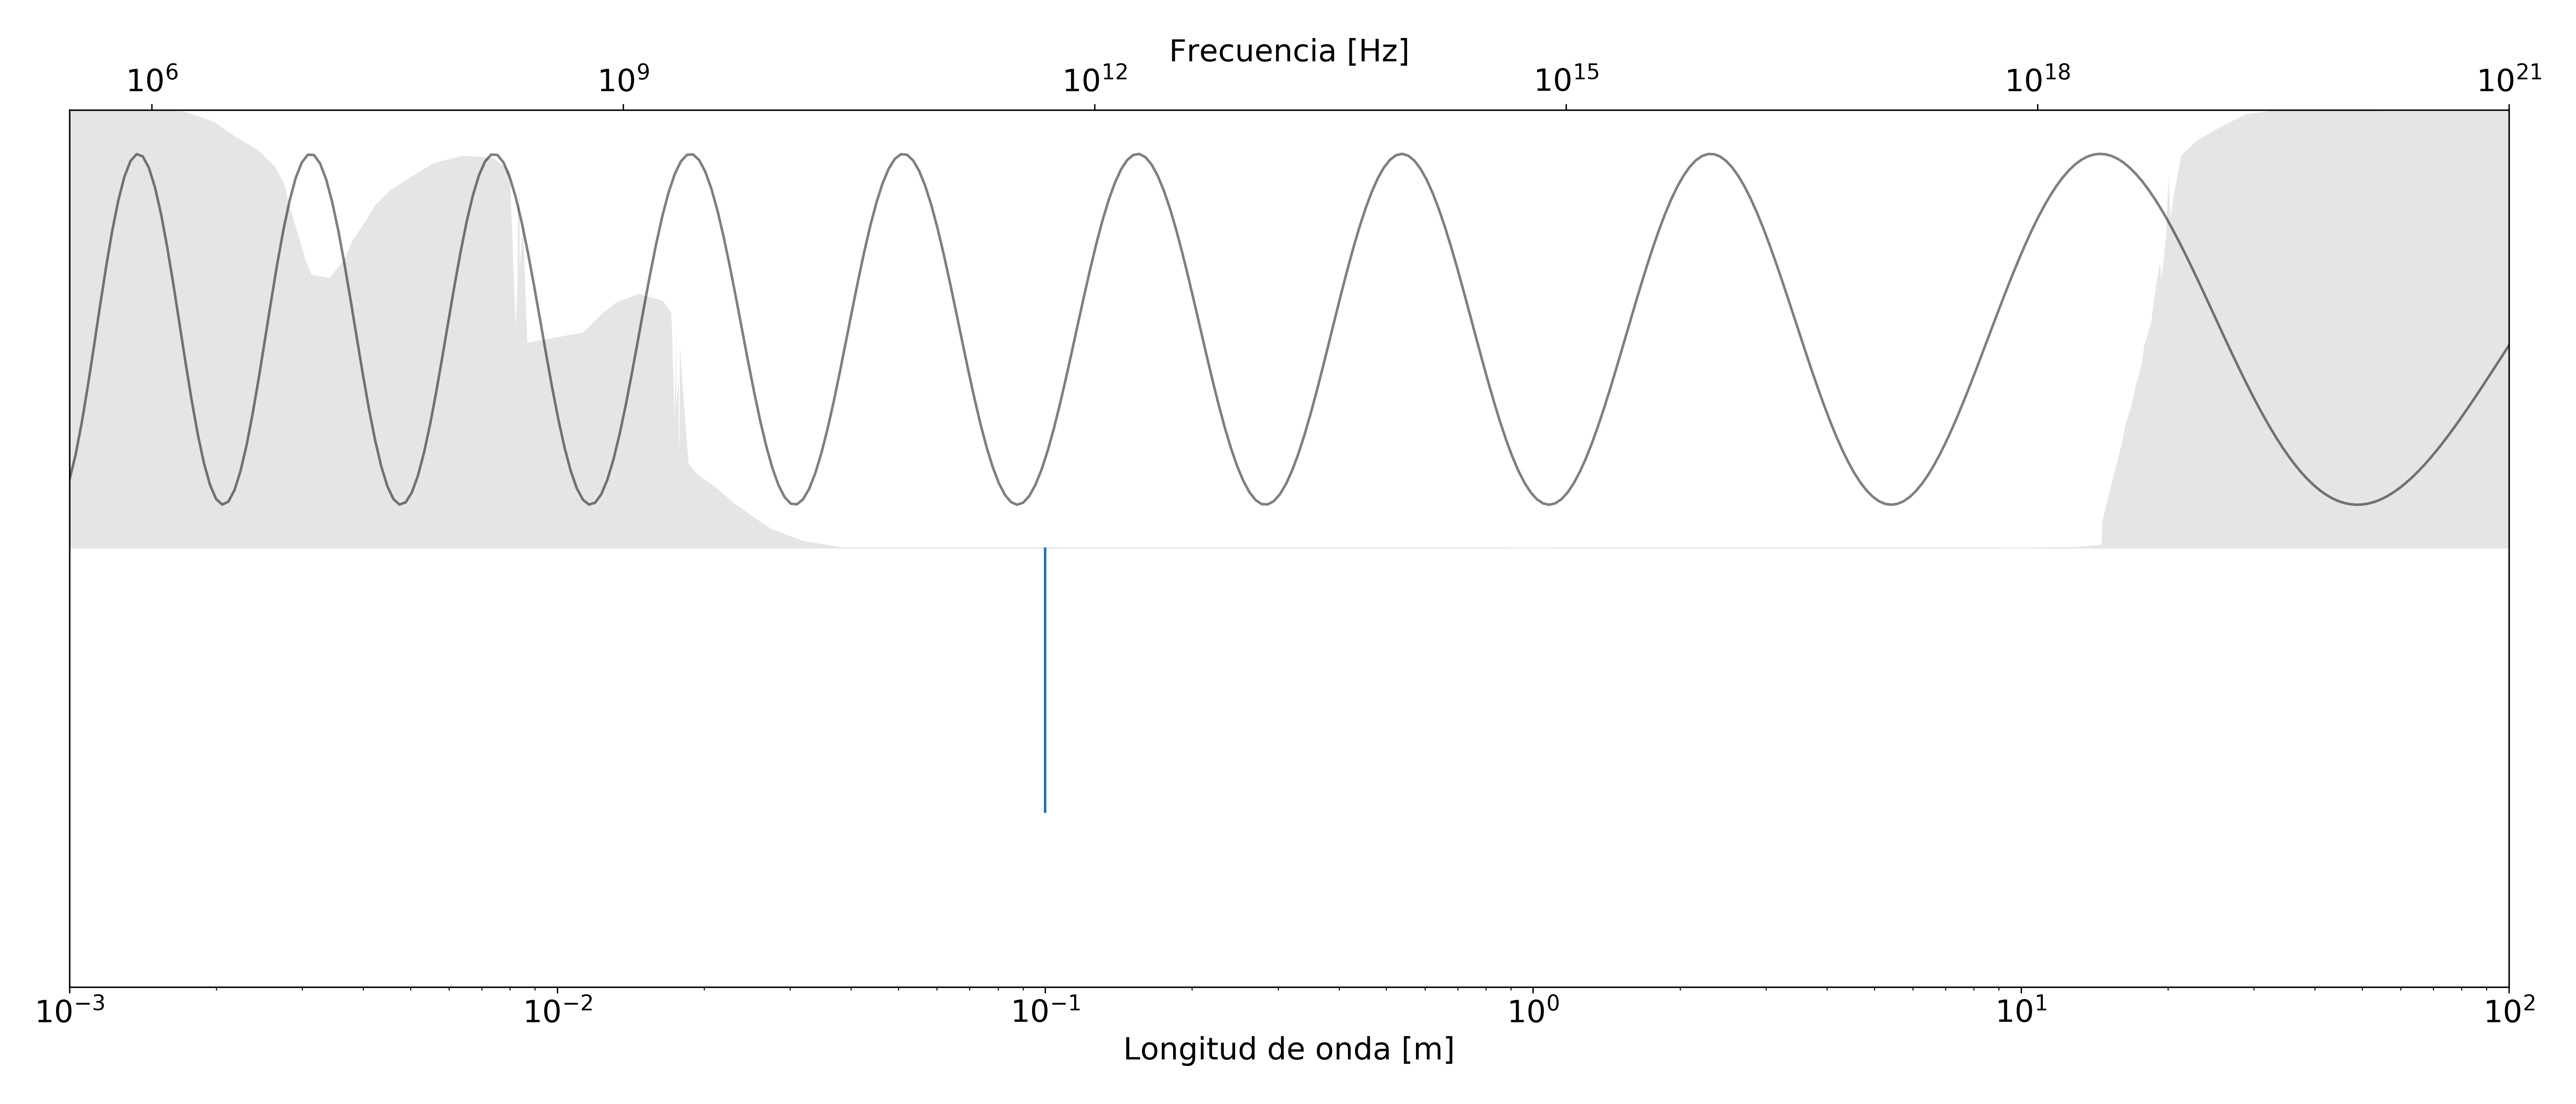
\includegraphics[width=\textwidth]{fig:espectro.png}
    \caption{Resolución espectral sobre la firma espectral.}
    \label{}
  \end{figure}
\end{frame}
%--- Next Frame ---%

\subsection{Proyección sobre el terreno}

\begin{frame}{\secname : \subsecname}
  \begin{figure}
    \centering
    %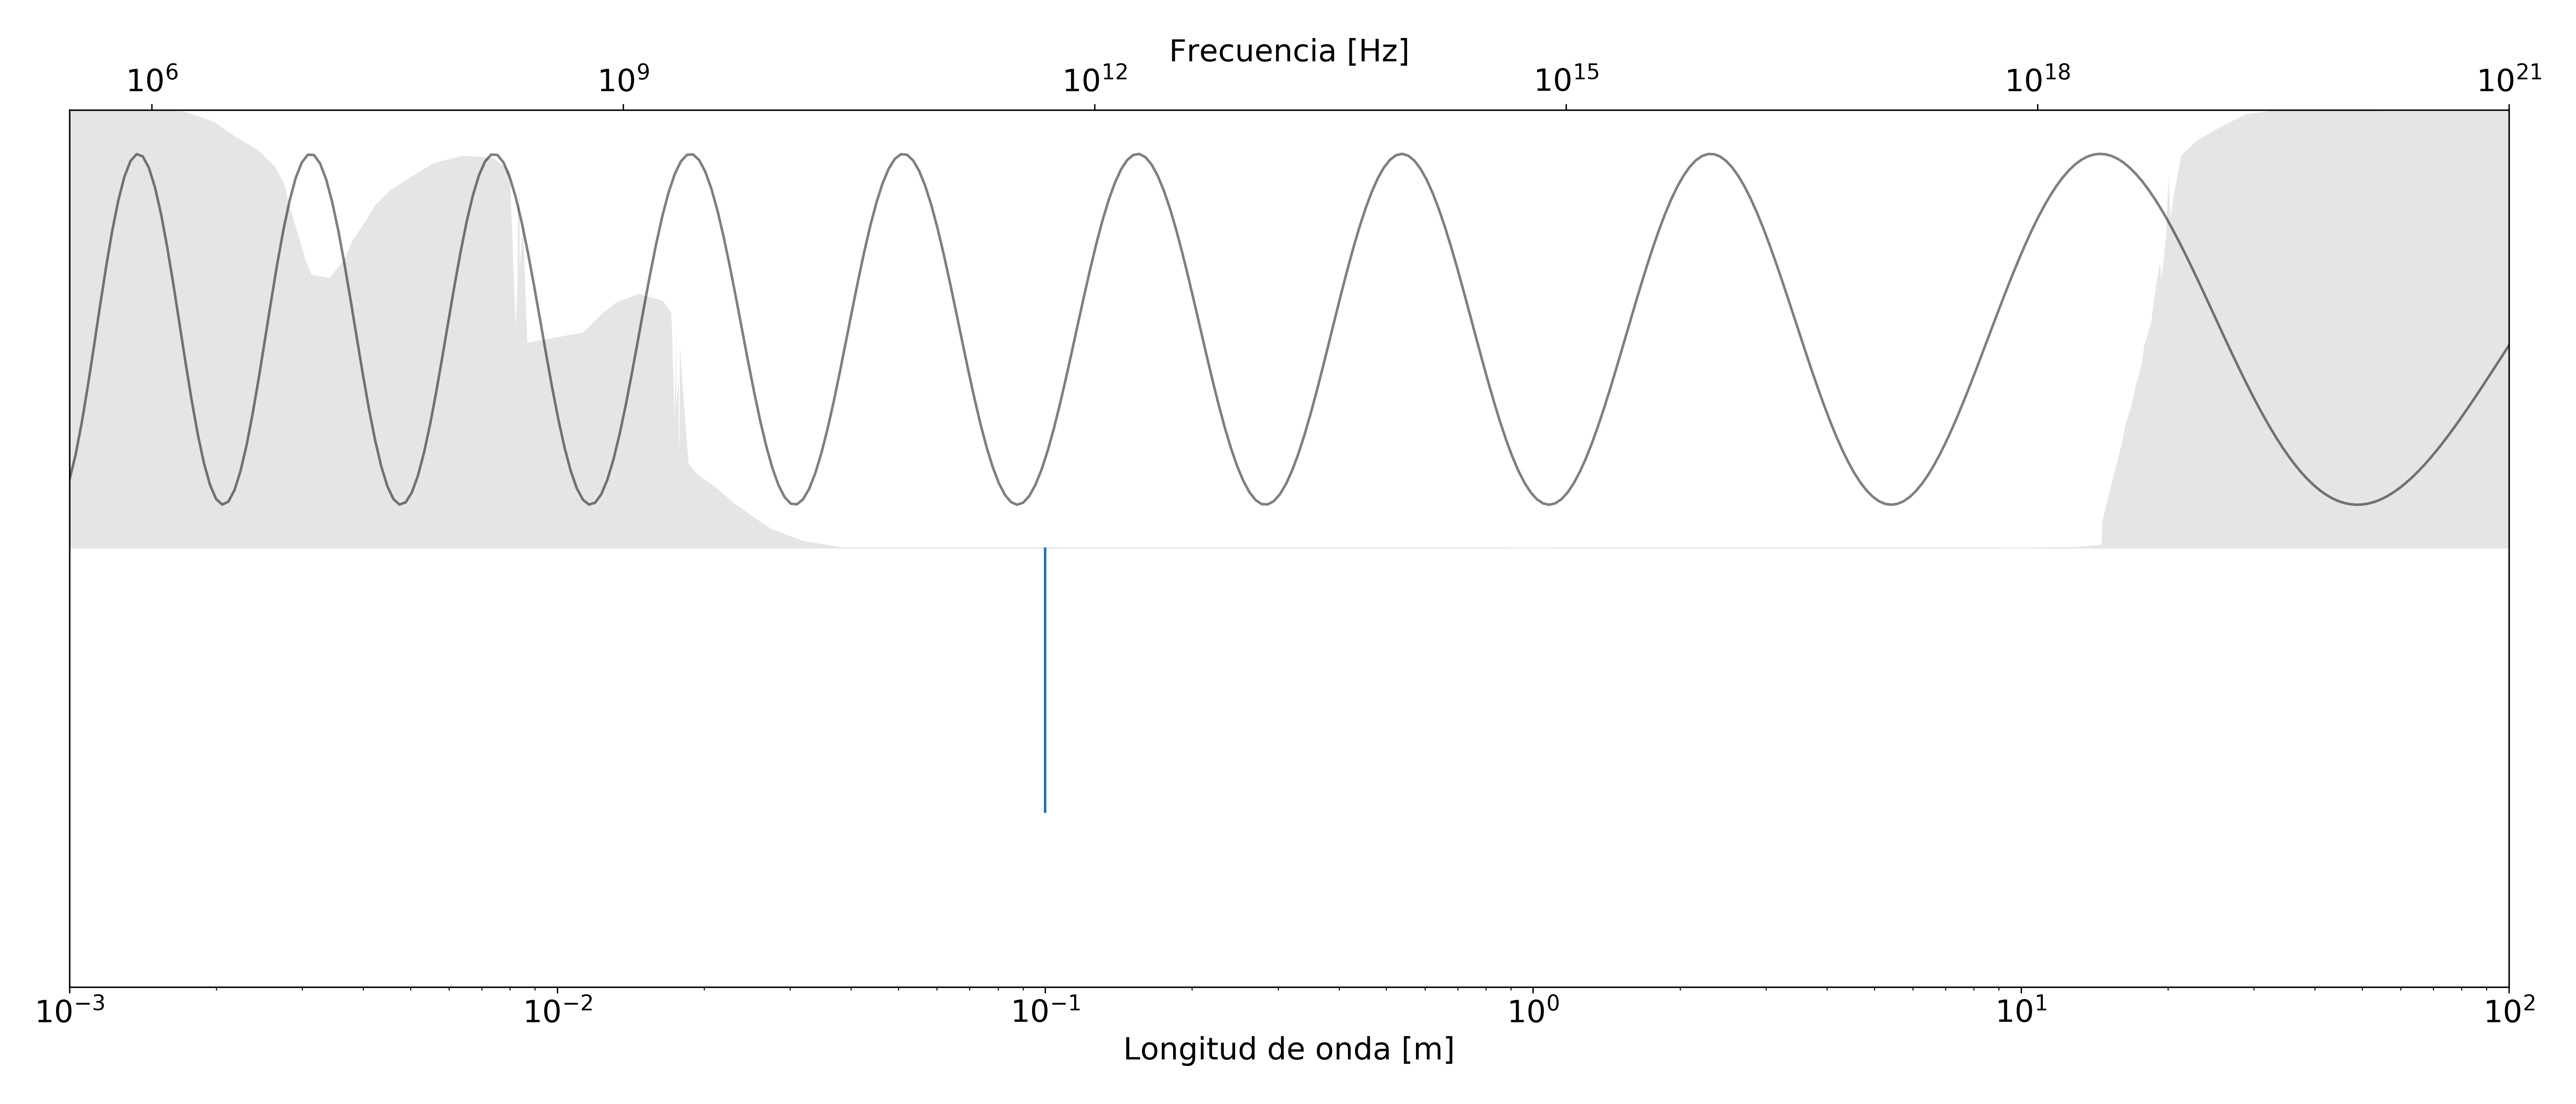
\includegraphics[width=\textwidth]{fig:espectro.png}
    \caption{Asignación de coordenadas a píxeles.}
    \label{}
  \end{figure}
\end{frame}
%--- Next Frame ---%

\begin{frame}{\secname : \subsecname}
  \begin{figure}
    \centering
    %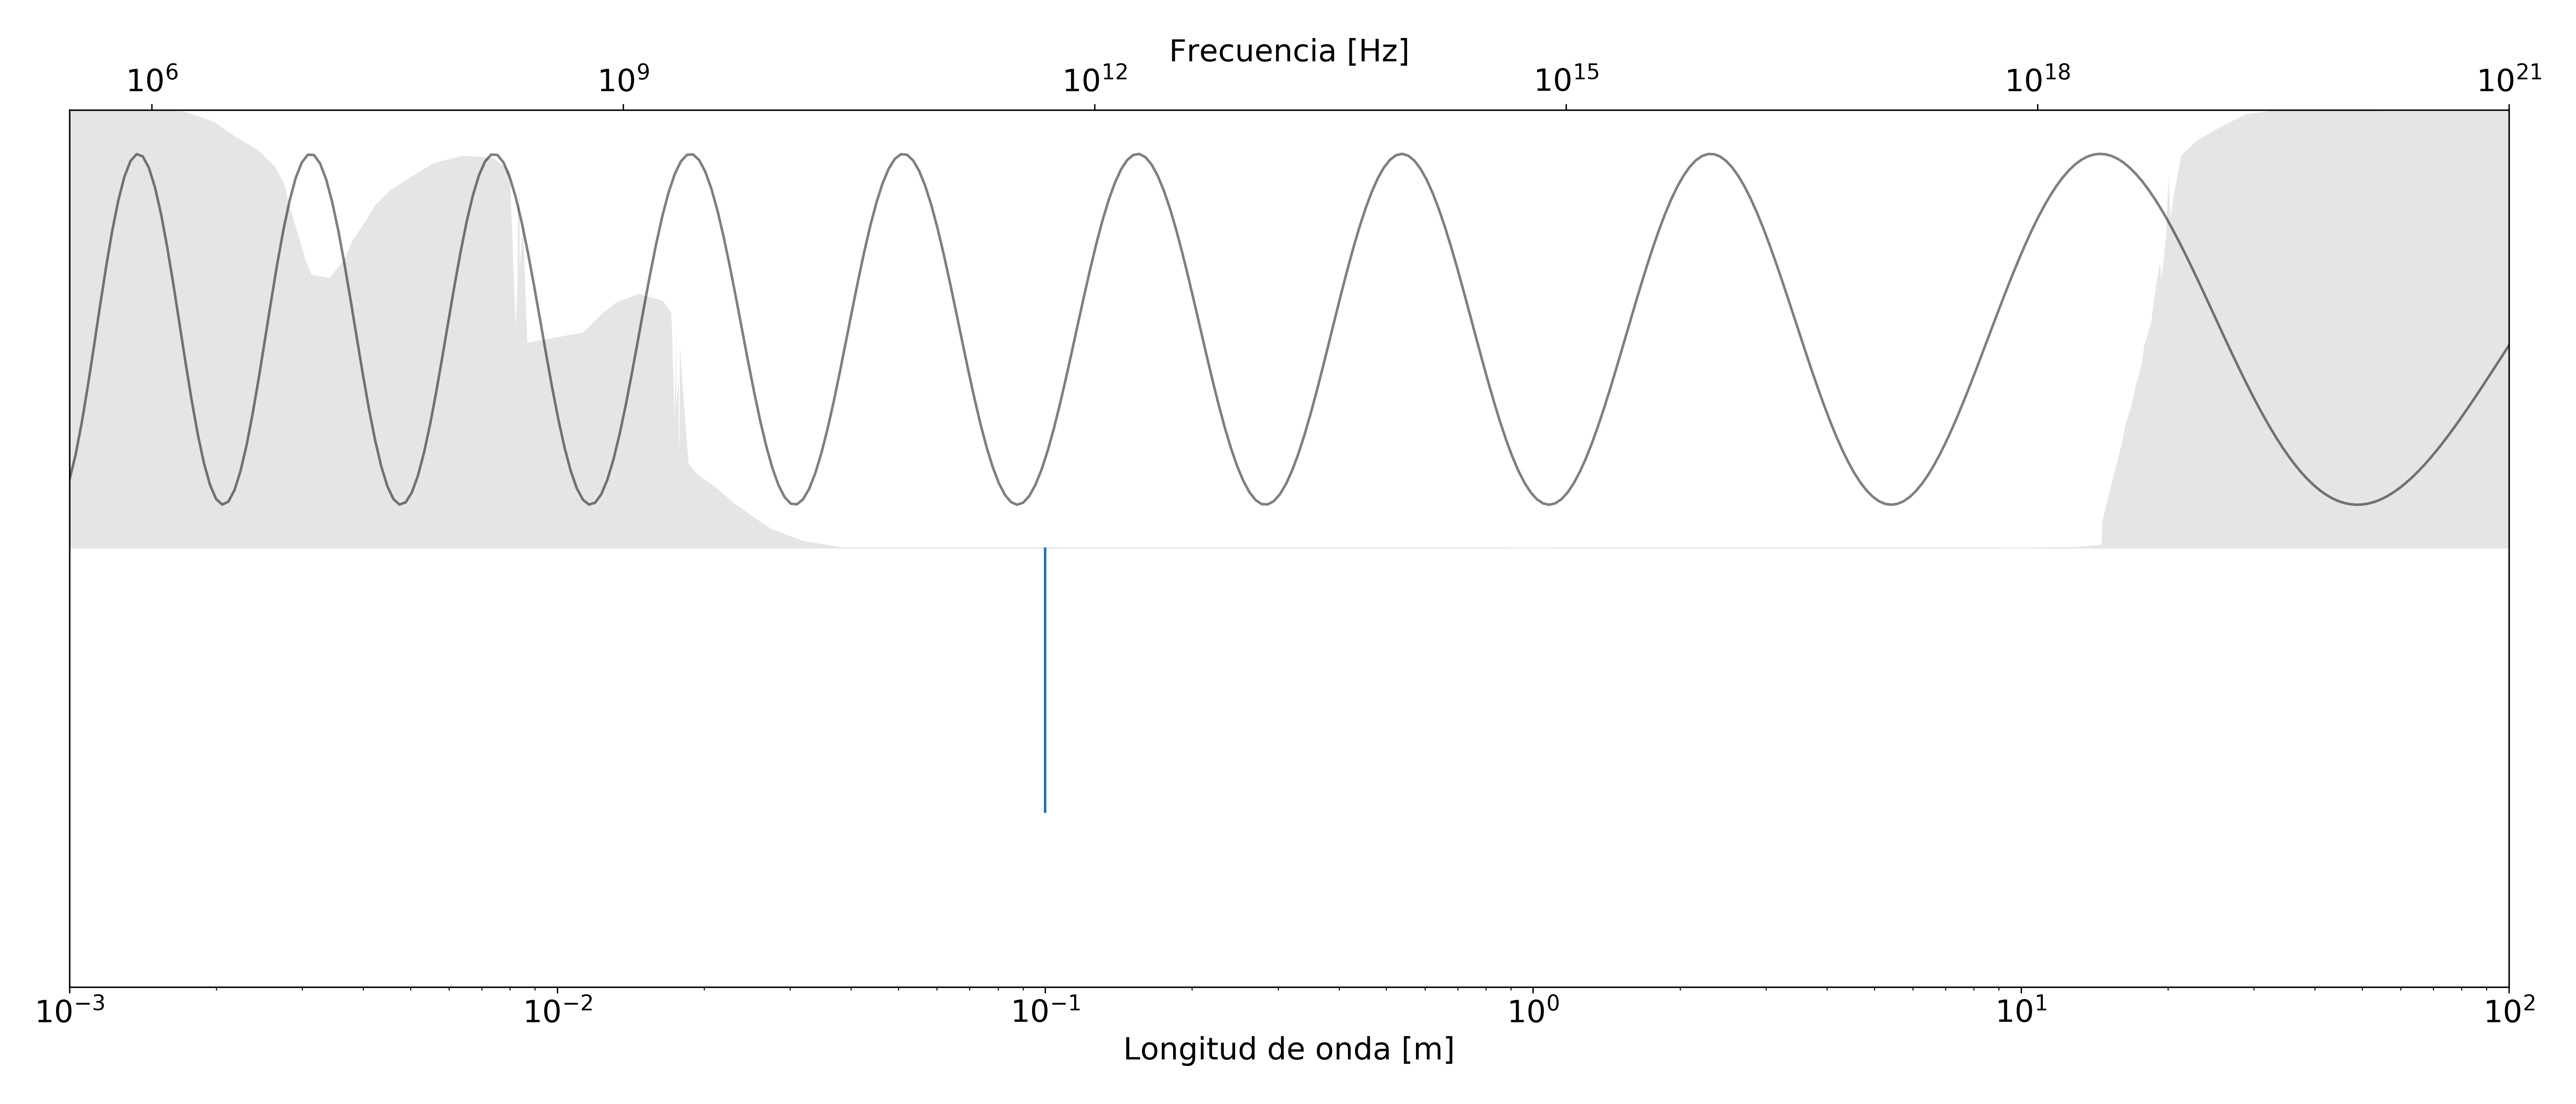
\includegraphics[width=\textwidth]{fig:espectro.png}
    \caption{Proyección de una esfera en un plano.}
    \label{}
  \end{figure}
\end{frame}
%--- Next Frame ---%

\begin{frame}{\secname : \subsecname}
  \begin{figure}
    \centering
    %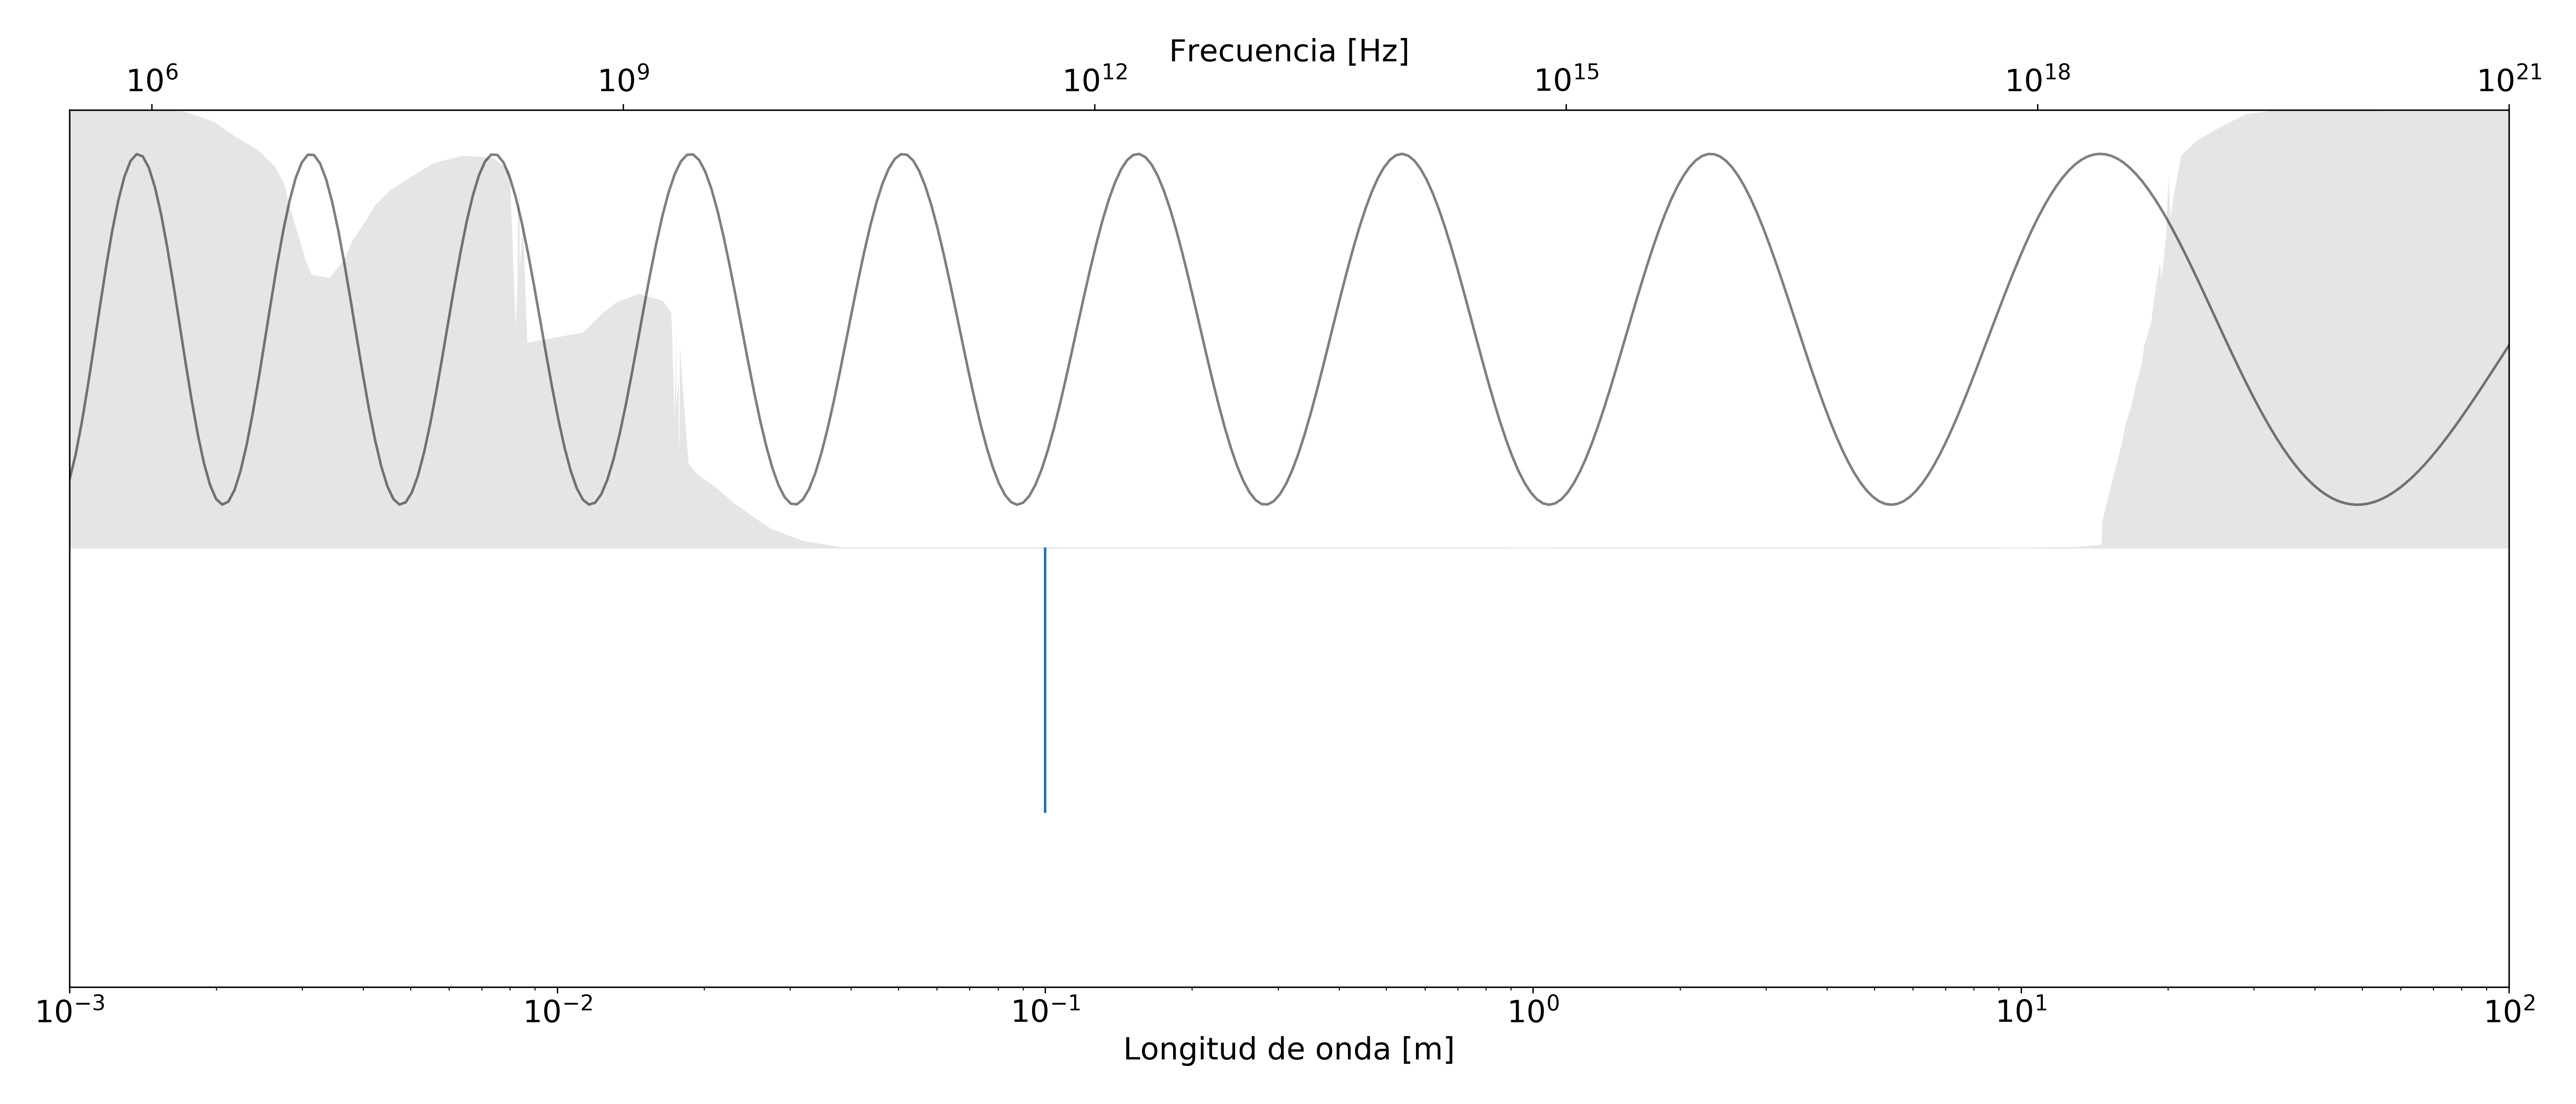
\includegraphics[width=\textwidth]{fig:espectro.png}
    \caption{Métodos de interpolación.}
    \label{}
  \end{figure}
\end{frame}
%--- Next Frame ---%

\begin{frame}{\secname : \subsecname}
  \begin{figure}
    \centering
    %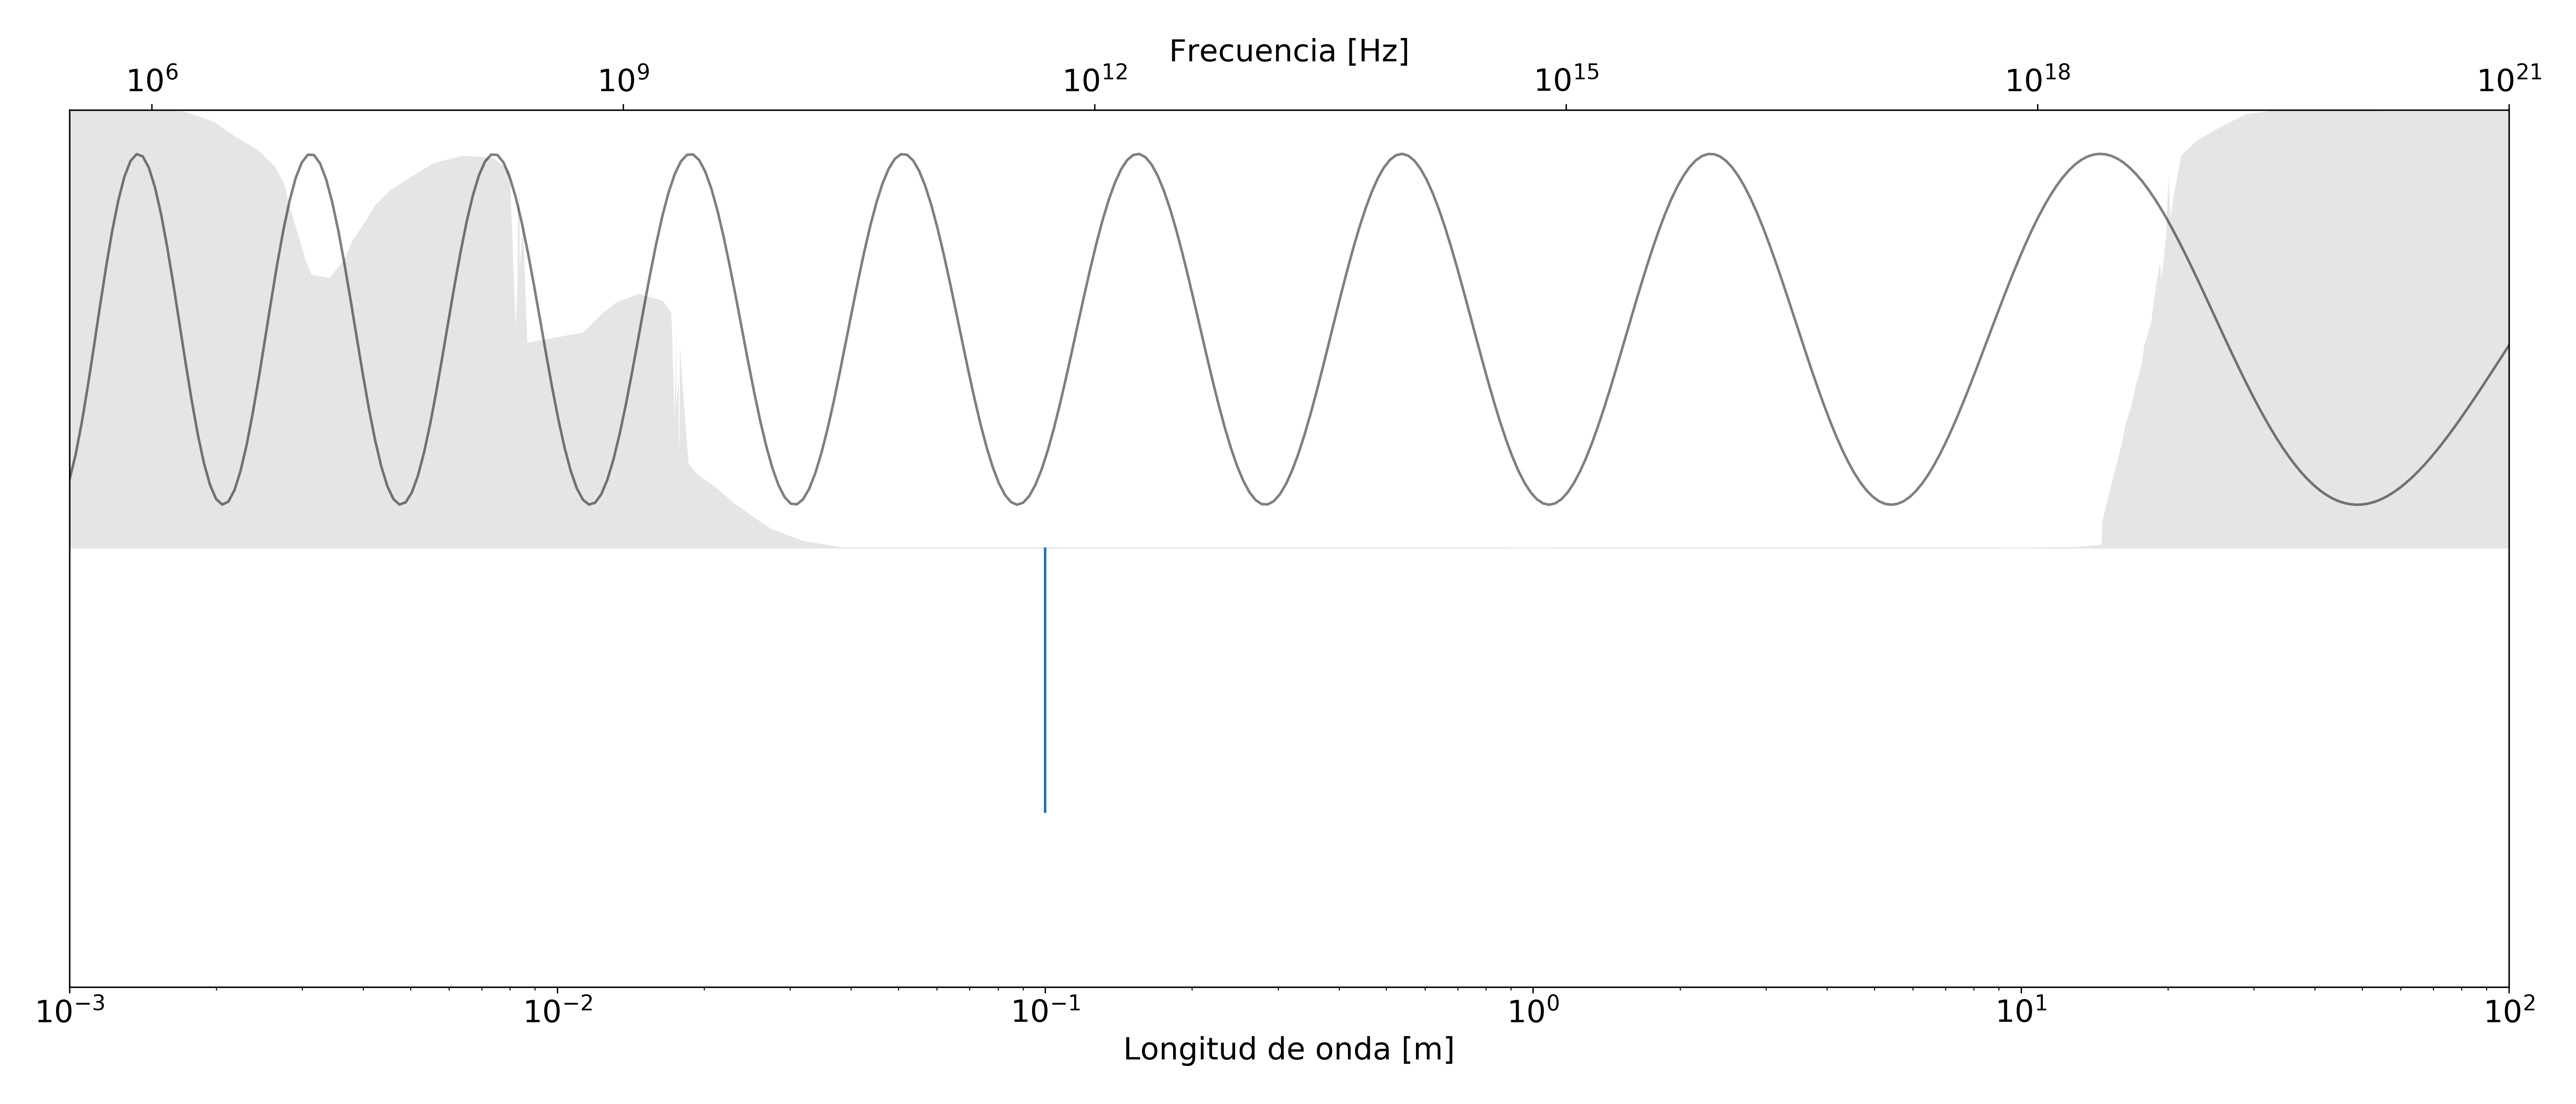
\includegraphics[width=\textwidth]{fig:espectro.png}
    \caption{Tipos de proyecciones.}
    \label{}
  \end{figure}
\end{frame}
%--- Next Frame ---%



\begin{frame}{\secname : \subsecname}
Muchas gracias.
\end{frame}
%--- Next Frame ---%
